% !TEX TS-program = pdflatex
% !TEX encoding = UTF-8 Unicode
% !TEX spellcheck = es_CL
% !TeX root=../Plantilla_PMT_MT.tex
% Creado por Fabián Inostroza 2015
 
\chapter{Introducción}

\section{Figuras}

Referencia a Figura~\ref{fig:simulaciones}. Referencia a subfigura~\ref{fig:sim1}.

\begin{figure}[h!tb]
\centering
\begin{subfigure}[b]{0.45\linewidth}
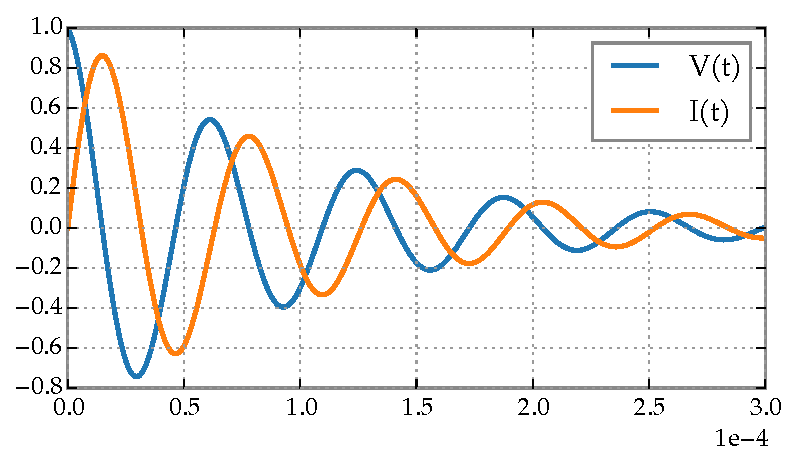
\includegraphics[width=\linewidth]{LC}
\caption{Simulación 1}
\label{fig:sim1}
\end{subfigure}
\begin{subfigure}[b]{0.45\linewidth}
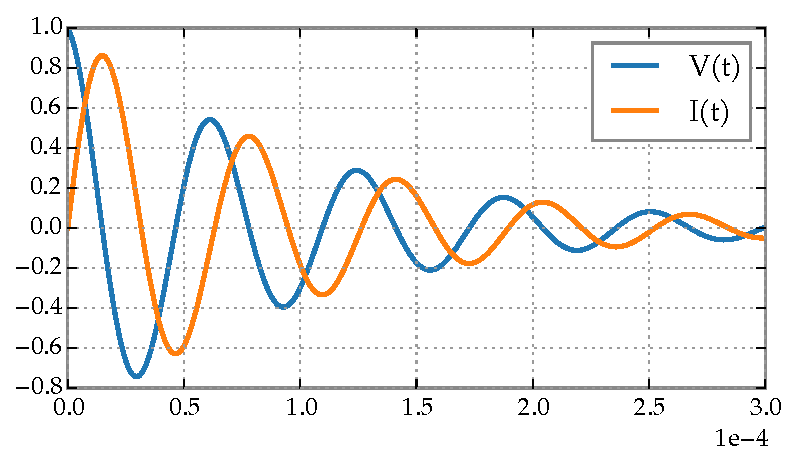
\includegraphics[width=\linewidth]{LC}
\caption{Simulación 2}
\label{fig:sim2}
\end{subfigure}

\begin{subfigure}[b]{0.7\linewidth}
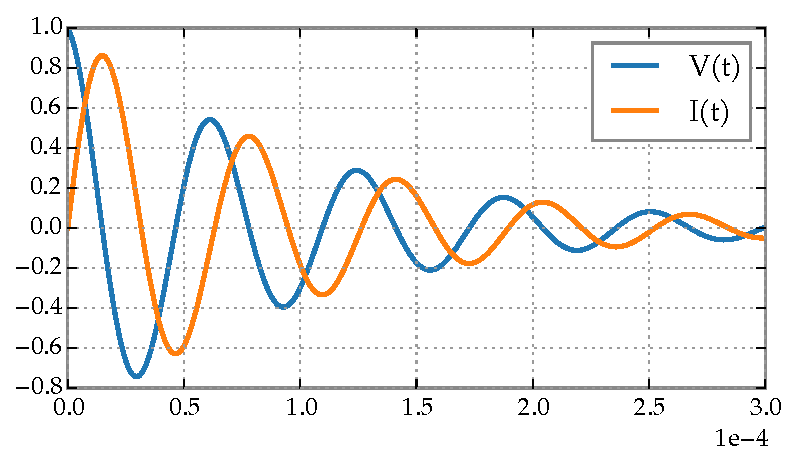
\includegraphics[width=\linewidth]{LC}
\caption{Simulación 3}
\label{fig:sim3}
\end{subfigure}

\caption{Ejemplo de subfiguras. Simulación 1~\subref{fig:sim1}, Simulación 2~\subref{fig:sim2} y Simulación 3~\subref{fig:sim3}.}
\label{fig:simulaciones}
\end{figure}

\section{Tablas}

\begin{table}[h!tb]
\centering
\caption{Ejemplo de tabla.}
\label{tab:ejemplo}
\begin{tabular}{ccccc}
\toprule
\multicolumn{2}{c}{Columna 1 y 2} & Columna 3 & Columna 4 & Columna 5 \\
\midrule
	Dato 1 & Dato 2 & Dato 3 & Dato 4 & Dato 5 \\
\cmidrule(r){1-2} \cmidrule(l){3-5}
	Dato 1 & Dato 2 & Dato 3 & Dato 4 & Dato 5 \\
\bottomrule
\end{tabular}
\end{table}


\section{Ecuaciones}
Ecuación alineada sin numerar
\begin{align*}
a &= b + c + d \\
e &= f + g + h + i
\end{align*}

Ecuación alineada numerada~\eqref{eq:num1},~\eqref{eq:num2}.
\begin{align}
a &= b + c + d \label{eq:num1} \\
e &= f + g + h + i \label{eq:num2}
\end{align}

Múltiples ecuaciones alineadas y con un solo número~\eqref{eq:num3}.
\begin{equation}
\begin{split}
\underbrace{a+\overbrace{b+\cdots}^{=t}+z}
_{\mathrm{total}} &= 
a+{\overbrace{b+\cdots}}^{126}+z \\
%% ecuacion 2
\underbrace{a+\overbrace{b+\cdots}^{=t}+z}
_{\mathrm{total}} &= 
a++b+{\overbrace{c+\cdots}}^{126}+z \\
\end{split}
\label{eq:num3}
\end{equation}

Matrices
\begin{align*}
\dot{\vect{x}} &= \vect{A}\vect{x} + \vect{B}\vect{u} \\
\dot{\vect{y}} &= \vect{C}\vect{x} + \vect{D}\vect{u}
\end{align*}

\begin{align*}
\vect{A} &= \begin{bmatrix}
1 & 0 & 0 \\
0 & 2 & 0 \\
0 & 0 & 3
\end{bmatrix}
%
&
%
\vect{B} &= \begin{bmatrix}
1  \\
0  \\
0 
\end{bmatrix}
%
&
%
\vect{C} &= \begin{bmatrix}
1 & 0 & 0 \\
0 & 2 & 0 \\
0 & 0 & 3
\end{bmatrix}
%
&
%
\vect{D} &= \begin{bmatrix}
1  \\
0  \\
0 
\end{bmatrix}
\end{align*}

\section{Listados de código}

\begin{lstlisting}[style=mlab, caption={código MATLAB.}]
function x = test(a, b)
  x = a + b;
end
\end{lstlisting}

\lstinputlisting[style=mlab, language=Python, caption={Código Python desde archivo.}, lastline=20]{figuras/tanque_LC.py}
